\item \textbf{{[}ALVL/9597/2017/P1/Q4{]} }

A computer program can generate a simple Sudoku puzzle using a 4 x
4 two-dimensional array. 

An example of this puzzle is: 
\begin{center}
\begin{tabular}{|c|c|c|c|}
\hline 
4 & 3 & 2 & 1\tabularnewline
\hline 
1 & 2 & 4 & 3\tabularnewline
\hline 
3 & 4 & 1 & 2\tabularnewline
\hline 
2 & 1 & 3 & 4\tabularnewline
\hline 
\end{tabular}
\par\end{center}

The first step to creating this puzzle is to develop a program to
display the 4 x 4 twodimensional array as a grid. This program will
display the grid as: 
\begin{center}
\begin{tabular}{cccc}
4 & 3 & 2 & 1\tabularnewline
1 & 2 & 4 & 3\tabularnewline
3 & 4 & 1 & 2\tabularnewline
2 & 1 & 3 & 4\tabularnewline
\end{tabular}
\par\end{center}

\subsubsection*{Task 4.1}

Create a program design that will declare, initialise and display
the example puzzle shown. This design will: 
\begin{itemize}
\item make use of top-down design 
\item include the data structure to represent the puzzle as a grid 
\item initialise the grid using the values shown
\item make use of appropriate procedures and/or functions. 
\end{itemize}

\subsubsection*{Evidence 13}

Your program design for Task 4.1. \hfill{}{[}6{]}

\subsubsection*{Task 4.2}

Write program code to display the puzzle designed in Task 4.1. 

\subsubsection*{Evidence 14}

Your program code.\hfill{} {[}5{]}

\subsubsection*{Evidence 15}

Screenshot of the displayed grid. \hfill{}{[}1{]}

The puzzle is said to be valid if it follows these rules:
\begin{itemize}
\item It consists of tour quadrants.
\item The numbers in each quadrant must add up to ten.
\item Each horizontal and vertical row of the puzzle must also add up to
ten.
\item No number can be repeated in the same row, same column or same quadrant
of the puzzle. 
\end{itemize}
A good strategy tor creating puzzles is to start with a valid \textquoteleft base'
puzzle and perform transformations on it to create new puzzles.

You will write program code to create new valid puzzles. 

Each puzzle created will have two randomly selected transformations.
from a possible four, performed on it. The following are the four
possible transformations that can be carried out. 
\begin{center}
\begin{tabular}{|c|>{\raggedright}p{0.3\columnwidth}|l|}
\hline 
\textbf{Transformation} & \texttt{\hspace{0.05\columnwidth}}Explanation & \multicolumn{1}{l}{}\tabularnewline
\hline 
\textbf{1} & Swaps two rows in the same quadrants & \tabularnewline
 &  & 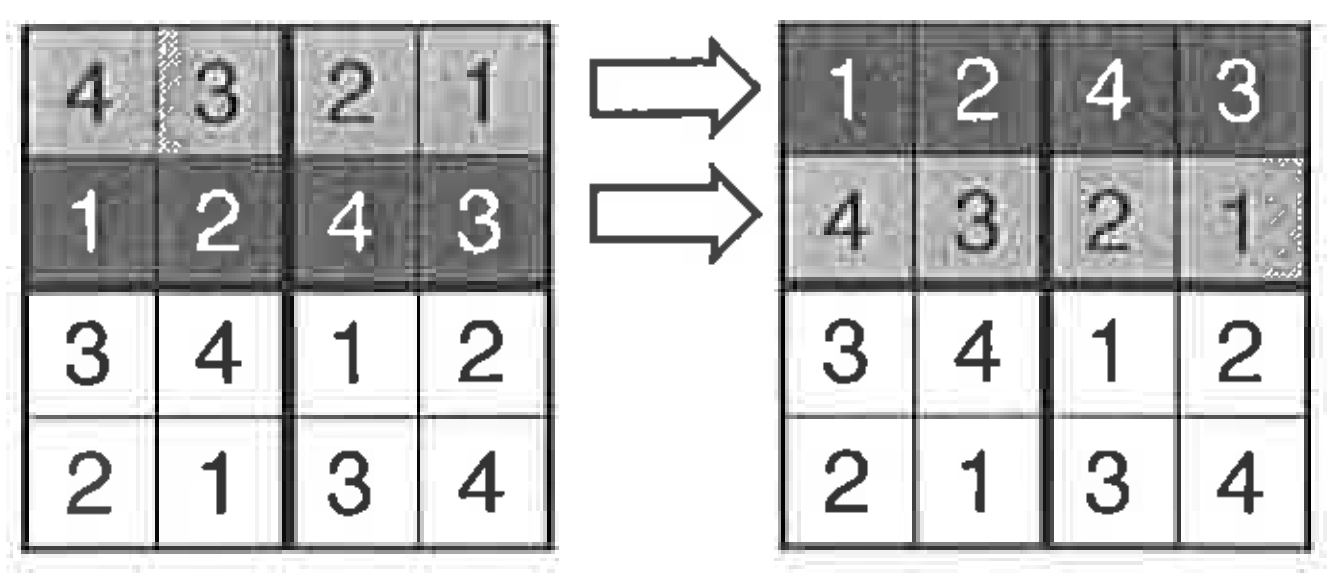
\includegraphics[width=0.3\paperwidth]{C:/Users/Admin/Desktop/Github/question_bank/LyX/static/img/9597-ALVL-2017-P1-Q4-1}\tabularnewline
\hline 
\textbf{2} & Swaps two columns in the same quadrants & \tabularnewline
 &  & 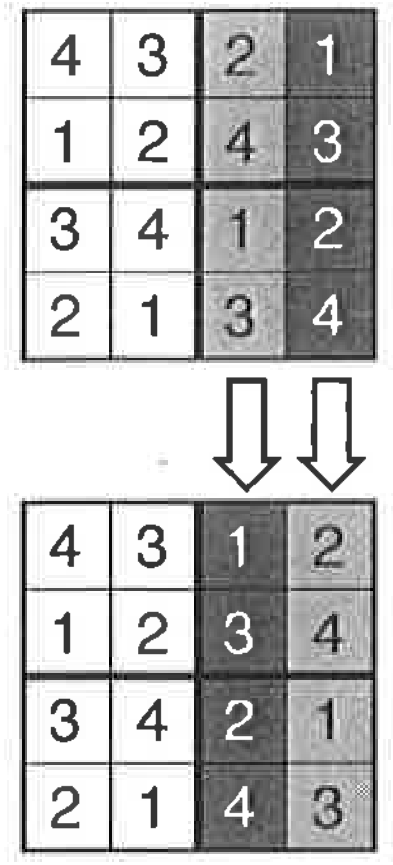
\includegraphics[width=0.15\paperwidth]{C:/Users/Admin/Desktop/Github/question_bank/LyX/static/img/9597-ALVL-2017-P1-Q4-2}\tabularnewline
\hline 
\textbf{3} & Swaps the top and bottom quadrant rows entirely & \tabularnewline
 &  & 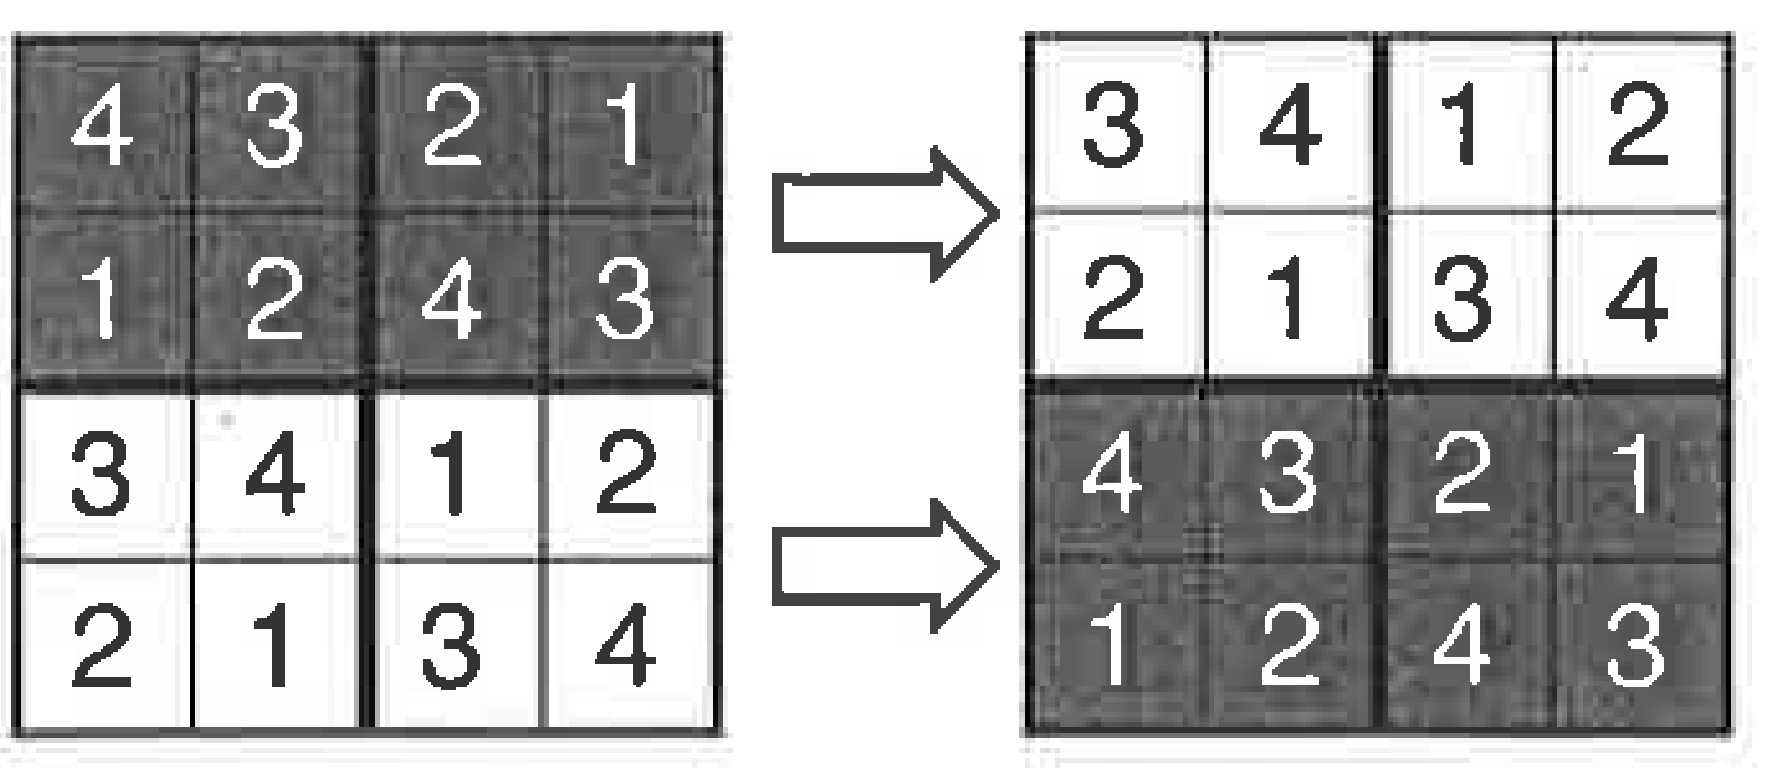
\includegraphics[width=0.3\paperwidth]{C:/Users/Admin/Desktop/Github/question_bank/LyX/static/img/9597-ALVL-2017-P1-Q4-3}\tabularnewline
\hline 
\textbf{4} & Swaps the left and right quadrant columns entirely & \tabularnewline
 &  & 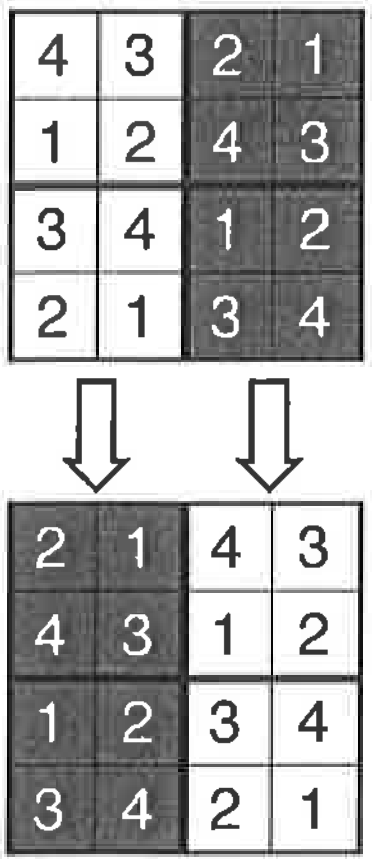
\includegraphics[width=0.15\paperwidth]{C:/Users/Admin/Desktop/Github/question_bank/LyX/static/img/9597-ALVL-2017-P1-Q4-4}\tabularnewline
\hline 
\end{tabular}
\par\end{center}

\subsubsection*{Task 4.3}

Write additional program code with brief \textbf{internal commentary}
to identify each transformation. 

The program code will: 
\begin{itemize}
\item create a method of selecting. at random, two of the four possible
transformations to be applied to the puzzle 
\item call a sub-program for each of the required transformations 
\item randomly select which rows will be transformed for transformations
1 and 2. for example. either the top or bottom two rows (for transformation
1) OR either the left-most or right-most two columns (for transformation
2) respectively 
\item display the puzzle before each transformation is applied and after
the final transformation. Before each transformation. it will also
display the name of the transformation being carried out. 

For example: 

\texttt{4321 }

\texttt{1243 }

\texttt{3412 }

\texttt{2134 }

\texttt{Transformation 1: Swaps two rows in the same quadrants }

\texttt{1243 }

\texttt{4321 }

\texttt{3412 }

\texttt{2134 }

\texttt{Transformation 4: Swaps the left and right quadrant columns
entirely }

\texttt{4312 }

\texttt{2143 }

\texttt{1234 }

\texttt{3421 }
\end{itemize}

\subsubsection*{Evidence 16}

Your program code that includes internal commentary.\hfill{} {[}14{]}

\subsubsection*{Evidence 17}

Screenshots of the output that shows each of the four transformations
applied. \hfill{}{[}4{]}